\chapter{Reflection and Conclusion}
\section{Planning and Management}
The plan of my project is divided into four parts:
\begin{enumerate}
    \item Read related research papers and prepare related knowledge and tools:
    
    Main research papers related to this project are \cite{pix2pix2016}, \cite{wang2018pix2pixHD},
    \cite{park2019SPADE}, I also spend time learning knowledge related to deep 
    learning and computer vision including CNN, ResNet, GAN, style transfer, etc. 
    Learning frameworks including Pytorch and Flask are also needed for implementation.
    \item Implement image translation models and trained them:
    
    This is the most difficult and time-consuming part of the project, I decided to implement 
    the two state-of-the-art models regarding image translation, however, it is not easy to 
    train such models on Colab because I do not have enough computing power, for example, 
    to duplicate the results mentioned in the paper of SPADE, the authors have trained the 
    network using eight Nvidia V100 GPUs for four days for one simulation, which is obviously 
    not practicable for me, not to mention the disconnecting issue. The solution here is to remove the unnecessary parts of 
    the project and choose a relatively small but still effective dataset for my implementation.
    \item Develop GUI for the project: 
    
    This is mainly a software engineering task, I have a similar experience using Spring framework 
    and Java for web development, so it is a relatively easy work for me to learn a similar 
    framework Flask for this project.
    \item Write report and record screencast: 
    
    The original plan is to start writing report once the demonstration(March 16th) is finished, 
    nevertheless, due to COVID-19 issue, I decided to travel back home on March 22nd, it took me 
    nearly a month before I can work on the report wholeheartedly.
\end{enumerate}

\begin{table}
    \begin{center}
    \begin{tabular}{|l|l|l|l|}\hline\hline
    To-Do&Planned Schedule&Actual Schedule\\
    \hline
    Background Preparation&Oct 01 - Nov 04&Oct 01 - Nov 07\\
    Train neural networks&Nov 04 - Feb 01&Nov 04 - Mar 16\\
    Develop Application&Feb 01 - Mar 02&Nov 04 - Mar 16\\
    Report and Screencast&Mar 16 - Apr 28&Apr 06 - May 05\\
    \hline\hline
    \end{tabular}
    \end{center}
    \caption{Schedule of 3rd Year Project}
    \label{milestones table}
\end{table}

Table \ref{milestones table} includes the to-do list for the project together with 
the originally planned timeline and the timeline that actually carried out. Several things 
were not carried out according to the original plan, the original plan was made 
before the arrangement of the lightening talk and demonstration, so I decided to start 
the training after I finished the lightening talk on November 7th. Apart from that, 
Since I have a lot of time waiting for the intermediate results during training, I decided
to merge the model training phase with the GUI development phase so that I can make 
full use of my time. For the last part of the project, I could not follow my original 
plan due to COVID-19 outbreak, and I cannot focus on writing the report before finishing
my quarantine and go back home, and fortunately, the deadline has also postponed.

\section{Future Works}
\label{sec:future work}
Due to computational resources and development time limitations, I am not able 
to implement all the functionalities mentioned in the paper of pix2pixHD\cite{wang2018pix2pixHD}
and SPADE\cite{park2019SPADE}, including:
\begin{itemize}
    \item Instance Maps in Pix2pixHD
    
    In segmentation maps, each pixel value represents a class of object, the maps will not 
    differentiate objects of the same category, e.g. if two cars stitch together in a 
    segmentation map, we are unable to know the boundaries of each car. On the other hand, 
    an instance map(or boundary map) will track each object with a unique ID. With the help 
    of instance maps, the model can deal the boundaries of objects better.
    \begin{figure}[H]
        \begin{center}
        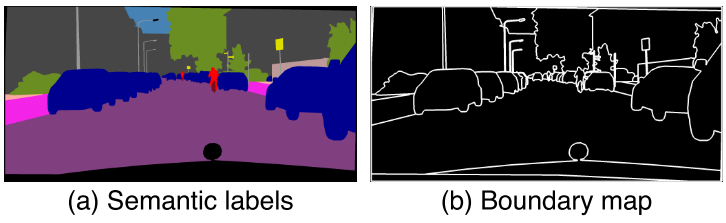
\includegraphics[width=8cm]{figures/instance-map}
        \end{center}
        \caption{Segmentation Map(a) VS. Instance Map(b)}
        \label{fig:instance-map}
    \end{figure}
    \item Variational Auto Encoder in SPADE
    
    As introduced in chapter 2, SPADE allows using a variational auto encoder to achieve 
    style transfer along with image translation. The encoder is consists of several 
    convolution blocks and convert the image into a mean vector $\mu$ and a variance vector
    $\sigma$, which is later used to calculate the noise input into the generator. 
    The VAE part needs separate training and tuning.
    \item Benchmark Datasets
    
    \nocite{zhou2016semantic}
    There are several benchmark datasets for image translation tasks including 
    Cityscapes \cite{Cordts2016Cityscapes}, ADE20K \cite{zhou2017scene}, etc. These 
    benchmark datasets provide much more training data than the one I use for 
    this project, which can check if the model can cope with complex scenes, i.e. test its ability of 
    translating segmentation maps with various objects(e.g. there are 20 classes of objects in Cityscapes) 
    or different kind of scenes(e.g. ADE20K contains houses scenes, art galleries scenes, airports 
    scenes, etc.). 
    However, it requires more computational resources to train networks on such 
    datasets.
    \item Hyperparameters Search
    
    It is desirable if we can search for the best hyperparameters for each model, this requires 
    training the networks multiple times(each time may take days). We might need some ways to 
    get some heuristics for hyperparameters combinations or it is not possible to iterate all 
    the possible options.
\end{itemize}

\section{Conclusion}
This project provides literature reviews on image-to-image translation topic
and experiments with two state-of-the-art image translation 
models with limited computational resources and compare their advantages and 
disadvantages. The experiments details have been written in jupyter notebooks 
and the implementation of the models are also wrapped up into a web app 
with a GUI so that people who are not familiar 
with this topic can check the experiments' process and results, and people
who have no ideas of coding and machine learning can also try image translation themselves.  

During this research and development process, I not only acquired a broad range of knowledge 
about deep learning and image translation, but also enhanced my self-learning skills. 
At first, I only knew some basic concepts of neural networks, then I learned how convolutional 
neural networks and its variations can solve those complex computer vision tasks, how to build a 
simple convolutional neural network myself with the help of deep learning frameworks. I read 
several papers regarding the image-to-image translation task, it is not easy to keep up with the 
novel ideas at first, but after searching for explanations from blogs or YouTube channels, I 
managed to get the ideas. Apart from that, I also practiced how to deploy machine learning 
models into a functional application like a web app.

In my perspective, even if the current state-of-the-art models can achieve 
astonishing results and are good enough for working prototypes, 
the approaches are still far from commercial uses.
First, the approaches still demand too many computation resources,
for example, if I want to duplicate image translation for the landscape dataset 
that the researchers did, I would still need eight Nvidia V100 GPUs training for days, which is not 
available for most of the users who just want to train a model for their specific domain. 
Another problem is that we have to provide enough training data for the model to work,
which is not necessarily as easy as it seems, for example, 
if we want to make a commercial application for designers to assist their designs, 
it is not easy to acquire novel designs as the training dataset.